\section{Results}

The results are split in two parts.
The first part is the context switching time value measured by our benchmarking framework.
For the second part, we have measured again the real context switching time with the oscilloscope the same way as for the reference measurement.

\subsection{Internal benchmarking framework results}
The value measured by our internal framework is represented in the table \ref{tab:internal-framework-measurement}.

\begin{table}[!ht]
  \centering
  \begin{tabular}{llll}
  & \multicolumn{3}{c}{Time ($\mu$s)}          \\ \cline{2-4} 
  & \multicolumn{1}{c}{Mean} & Min  & Max  \\ \cline{2-4} 
From task 1 to task 2 & 7812                     & 7812 & 7812 \\
From task 2 to task 1 & 7812                     & 7812 & 7812
\end{tabular}
  \caption{Context switching time measured by our internal benchmarking framework}
  \label{tab:internal-framework-measurement}
  \end{table}

\subsection{External benchmarking framework results}
The context switching time computed by our external framework is displayed in the table \ref{tab:external-framework-measurement}.

\begin{table}[!ht]
  \centering
  \begin{tabular}{llll}
  & \multicolumn{3}{c}{Time ($\mu$s)}                             \\ \cline{2-4} 
  & \multicolumn{1}{c}{Mean} & Min  & \multicolumn{1}{c}{Max} \\ \cline{2-4} 
Context switching time & 18.93                     & 15.62 & 40.26                    \\
\end{tabular}
  \caption{Context switching time measured by our external benchmarking framework}
  \label{tab:external-framework-measurement}
\end{table}

\subsection{Oscilloscope results}
Using the same setup as for the reference measurement, we have measured again the real context switching time with both our internal and external benchmarking framework.

The figure \ref{fig:internal-framework-value-wave} shows the voltage measurement of the two GPIOs used by the tasks while using our internal framework.
The figure \ref{fig:external-framework-value-wave} shows the voltage measurement of the single GPIO used by the external framework while using it.

\begin{figure}[!ht]
  \centering

  \begin{minipage}{0.45\textwidth}
    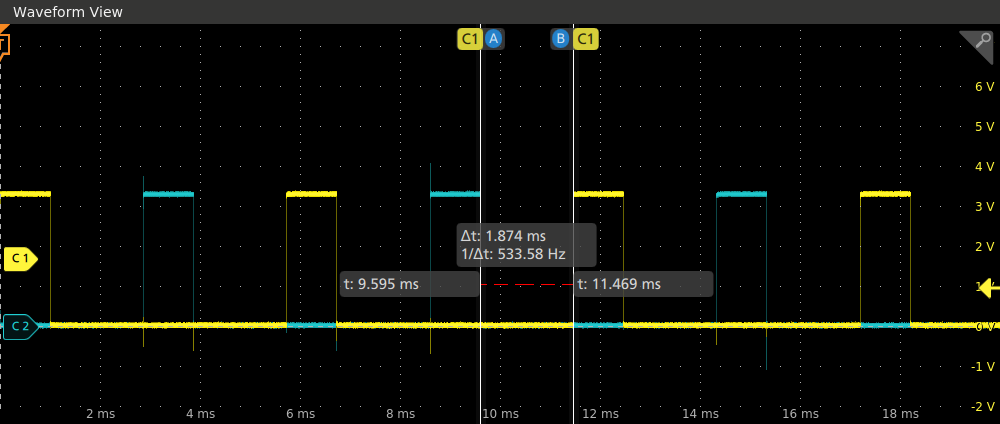
\includegraphics[width=0.9\textwidth]{assets/framework-value-wave.png}
    \caption{\label{fig:internal-framework-value-wave}Internal benchmarking framework voltage measurement}

  \end{minipage}\hfill
  \begin{minipage}{0.45\textwidth}

    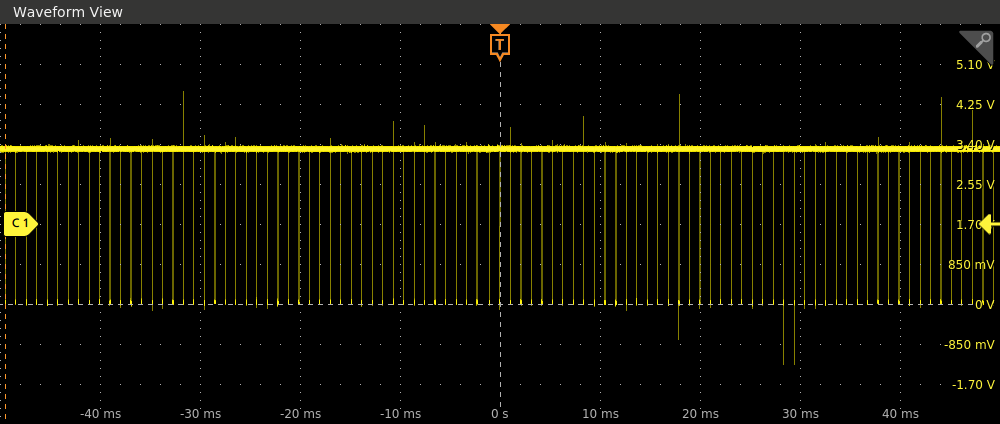
\includegraphics[width=0.9\textwidth]{assets/external-framework-value-wave.png}
    \caption{\label{fig:external-framework-value-wave}External benchmarking framework voltage measurement}

  \end{minipage}
\end{figure}

The table \ref{tab:frameworks-oscilloscope-comparison} shows a comparison of the real context switching time measured with the oscilloscope between the internal framework and the external one.

\begin{table}[!ht]
  \centering
  \begin{tabular}{llllllll}
  & \multicolumn{7}{c}{Time ($\mu$s)}                                                      \\ \cline{2-8} 
  & \multicolumn{3}{c}{Internal framework} &  & \multicolumn{3}{c}{External framework} \\ \cline{2-4} \cline{6-8} 
  & \multicolumn{1}{c}{Mean} & Min  & Max  &  & Mean        & Min         & Max        \\ \cline{2-4} \cline{6-8} 
Context switching time & 1865                     & 1862 & 1866 &  & 14.87       & 14.79       & 14.97      \\
Duration of task 1     & 1003                     & 1003 & 1003 &  & 1003        & 1003        & 1003       \\
Duration of task 2     & 1003                     & 1003 & 1003 &  & 1003        & 1003        & 1003      
\end{tabular}
  \caption{Context switching times and task durations measured with the oscilloscope using our internal and external benchmarking frameworks}
  \label{tab:frameworks-oscilloscope-comparison}
\end{table}

\subsection{Discussions}

\subsubsection{Internal benchmarking framework}

By comparing with our reference measurement, the first assessment we can make is that our benchmarking framework does not compute the context switching time correctly.
The framework measure a context switching time of 7812 $\mu$s where we expect a value of 14.68 $\mu$s.

Second assessment we can make is that our framework add a huge overhead.
When comparing the figure \ref{fig:measurement-value-wave} with the figure \ref{fig:internal-framework-value-wave}, the overhead is largely visible.
By comparing the values measured by the oscilloscope, the reference measurement and the real context switching time while using our framework, we see that our framework add an overhead of 1850 $\mu$s.
The table \ref{tab:measurements-comparison} shows this comparison.

\begin{table}[!ht]
  \centering
  \begin{tabular}{lll}
                        & \multicolumn{2}{c}{Time ($\mu$s)}                                     \\ \cline{2-3} 
                        & \multicolumn{1}{c}{No framework} & Framework \\ \cline{2-3} 
  From task 1 to task 2 & 14.68                                     & 1864                  \\
  From task 2 to task 1 & 14.88                                     & 1865                  \\
  Duration of task 1    & 1003                                      & 1003                  \\
  Duration of task 2    & 1003                                      & 1003                 
  \end{tabular}
  \caption{Comparison of the oscilloscope measurements}
  \label{tab:measurements-comparison}
\end{table}

\paragraph{}{Limitations of the framework}
As the results show, our framework suffers from several limitations.

First, the devices can not compute the context switching time with enough precision.
This lack of precision is due of the speed of the device clock that is not high enough.
In our experiment, the Zolertia RE-MOTE used with Contiki could only use a timer with 128 ticks per second or 1 tick every 7812 $\mu$s.

Second, our framework output its computed value through serial port.
Printing out at least 32 characters for every context switch on the serial port even at 250 kbit/s took 1.2ms.
One optimization could be to reduce the number of bits send or use a cache.

\subsubsection{External benchmarking framework}

The first thing we can see is that our external benchmarking framework is much more precise that our internal benchmarking framework.
Even if the result does not match our excpectation, the results show an improvement.
We went from a measurement error with a factor of more than 500 to a measurement error with a factor less than 2.

Secondly, with the real context switching time measured at 14.87$\mu$s while our framework was on, our external benchmarking framework does not add an overhead.

In conclusion, our external benchmarking framework is more precise than our internal benchmarking framework and does not add an overhead to the real context switching time.